% =================================================
% HOVEDDOKUMENT (NOTATMAL)
% =================================================
%
% Langformede notater i teoretisk fysikk og matematikk.
%
% Det typografiske utseendet er definert i notesstyle.sty
% og bør ikke endres her.
%
% =================================================


\documentclass[a4paper,11pt]{article}


% =================================================
% LAST INN NOTATSTIL
% =================================================
\usepackage{notatstil}


% =================================================
% SPRÅK
% =================================================
\usepackage[norsk]{babel}


% =================================================
% EGENDEFINERTE PAKKER
%
% Legg til prosjektspesifikke pakker her.
% Ikke sett pakker andre steder i filen.
% =================================================

% --- Matematikk (standard) ---
\usepackage{amsmath, amssymb, amsthm}
\usepackage{mathtools}

% --- Valgfrie fysikk- / matematikkutvidelser ---
% \usepackage{physics}              % \dd, \ket, \bra, \comm, ...
% \usepackage{bm}                   % uthevede mattesymboler
% \usepackage{slashed}              % Feynman-skråstrek
% \usepackage{tensor}               % indekserte tensorer

% --- Annet ---
\usepackage{graphicx}               % figurer
\graphicspath{{figurer/}}           % figurer ligger i figurer/
\usepackage{booktabs}               % tabeller
% \usepackage{enumitem}             % listetilpasning


% =================================================
% TEOREMOMGIVELSER
% =================================================
\theoremstyle{plain}
\newtheorem{teorem}{Teorem}[section]

\theoremstyle{definition}
\newtheorem{definisjon}[teorem]{Definisjon}

\theoremstyle{remark}
\newtheorem{merknad}[teorem]{Merknad}

% Norsk navn på proof-omgivelsen
\renewcommand{\proofname}{Bevis}


% =================================================
% EGENDEFINERTE KOMMANDOER
%
% Prosjektspesifikke makroer.
% =================================================

% \newcommand{\dd}{\mathrm{d}}
% \newcommand{\ii}{\mathrm{i}}


% =================================================
% METADATA
% =================================================
\title{Notattittel}
\author{Forfatternavn}
\date{\today}


% =================================================
% DOKUMENT
% =================================================
\begin{document}

\maketitle

\begin{abstract}
Et kort sammendrag som introduserer innholdet i disse notatene.
\end{abstract}

\tableofcontents
\clearpage


% =================================================
\section{Bakgrunn}

Disse notatene utvikler en liten bit av teoretisk maskineri
for å illustrere strukturen i malen. Fremstillingen følger
det typiske mønsteret for matematikk- og fysikknotater:
definisjoner, formuleringer av resultater, korte bevis, og
gjennomgåtte eksempler vekslet med prosa.

Siteringer vises i hakeparenteser, f.eks.\ \cite{eksempel-artikkel},
og flere kilder kombineres og komprimeres til intervaller
automatisk~\cite{eksempel-artikkel,eksempel-bok}.


% =================================================
\section{Definisjoner og resultater}

\begin{definisjon}
  La $\mathcal{H}$ være et komplekst separabelt Hilbertrom. En
  \emph{tilstand} er en enhetsvektor $\psi \in \mathcal{H}$,
  betraktet opp til en fasefaktor $e^{i\theta}$.
\end{definisjon}

\begin{definisjon}
  En \emph{observabel} er en selvadjungert lineær operator
  $\hat{A}$ som virker på $\mathcal{H}$.
\end{definisjon}

Forventningsverdien til en observabel i en gitt tilstand er
definert ved
\begin{equation}
  \langle A \rangle_\psi
  = \langle \psi | \hat{A} | \psi \rangle .
  \label{eq:forventning}
\end{equation}

\begin{teorem}
  Forventningsverdier av selvadjungerte operatorer er reelle.
\end{teorem}

\begin{proof}
  Per definisjon,
  $\overline{\langle A \rangle_\psi}
  = \overline{\langle \psi | \hat{A} | \psi \rangle}
  = \langle \psi | \hat{A}^\dagger | \psi \rangle
  = \langle \psi | \hat{A} | \psi \rangle
  = \langle A \rangle_\psi$,
  hvor vi brukte $\hat{A}^\dagger = \hat{A}$.
\end{proof}

\begin{merknad}
  At forventningsverdier er reelle, er det som gjør
  selvadjungerte operatorer til den naturlige matematiske
  modellen for observerbare størrelser i kvantemekanikk.
\end{merknad}

\subsection{Tidsutvikling}

Tidsutvikling i kvantemekanikk styres av Schr\"odinger-ligningen:
\begin{equation}
  i\hbar \frac{\partial \psi}{\partial t}
  = \hat{H}\psi ,
  \label{eq:schrodinger}
\end{equation}
hvor $\hat{H}$ er Hamilton-operatoren. For tidsuavhengig
$\hat{H}$ integrerer ligning~\eqref{eq:schrodinger} til
\begin{equation}
  \psi(t) = e^{-i\hat{H}t/\hbar}\,\psi(0).
\end{equation}


% =================================================
\section{Eksempler}

\begin{figure}[t]
  \centering
  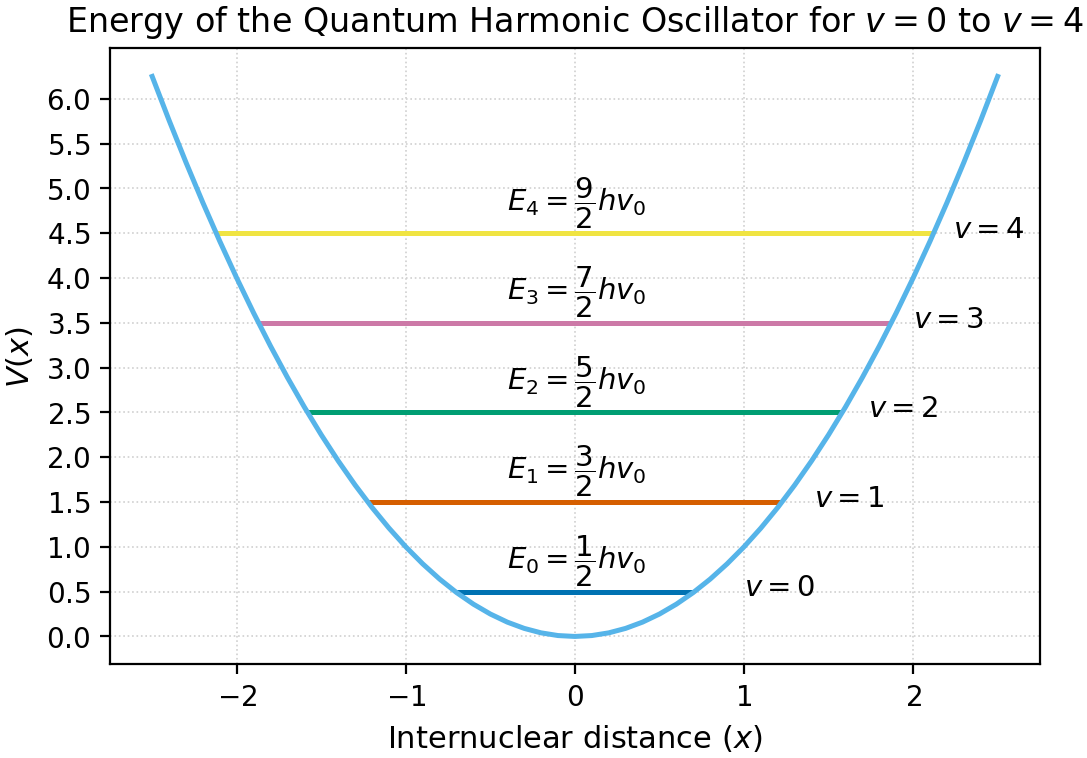
\includegraphics[width=0.7\linewidth]{Energy_levels}
  \caption{Skjematisk energinivådiagram.}
  \label{fig:nivaer}
\end{figure}

Figur~\ref{fig:nivaer} viser en typisk struktur som dukker
opp gjennom resten av notatene.

\begin{table}[t]
  \centering
  \caption{Fundamentale fysiske konstanter.}
  \label{tab:konstanter}
  \begin{tabular}{lcr}
    \toprule
    Størrelse           & Symbol  & Verdi                         \\
    \midrule
    Lysets hastighet    & $c$     & $2{,}998 \times 10^8$ m/s     \\
    Plancks konstant    & $\hbar$ & $1{,}055 \times 10^{-34}$ Js  \\
    Elementærladning    & $e$     & $1{,}602 \times 10^{-19}$ C   \\
    \bottomrule
  \end{tabular}
\end{table}


% =================================================
\section{Avslutning}

Disse notatene er en mal; innholdet over finnes kun for å
demonstrere typografi. Bytt det ut med ditt eget materiale
etter hvert som notatene utvikler seg.


% =================================================
% BIBLIOGRAFI
% =================================================
\bibliographystyle{unsrtnat}
\bibliography{referanser}


\end{document}
